\documentclass[sn-apa]{sn-jnl}\usepackage[]{graphicx}\usepackage[]{xcolor}
% maxwidth is the original width if it is less than linewidth
% otherwise use linewidth (to make sure the graphics do not exceed the margin)
\makeatletter
\def\maxwidth{ %
  \ifdim\Gin@nat@width>\linewidth
    \linewidth
  \else
    \Gin@nat@width
  \fi
}
\makeatother

\definecolor{fgcolor}{rgb}{0.345, 0.345, 0.345}
\newcommand{\hlnum}[1]{\textcolor[rgb]{0.686,0.059,0.569}{#1}}%
\newcommand{\hlstr}[1]{\textcolor[rgb]{0.192,0.494,0.8}{#1}}%
\newcommand{\hlcom}[1]{\textcolor[rgb]{0.678,0.584,0.686}{\textit{#1}}}%
\newcommand{\hlopt}[1]{\textcolor[rgb]{0,0,0}{#1}}%
\newcommand{\hlstd}[1]{\textcolor[rgb]{0.345,0.345,0.345}{#1}}%
\newcommand{\hlkwa}[1]{\textcolor[rgb]{0.161,0.373,0.58}{\textbf{#1}}}%
\newcommand{\hlkwb}[1]{\textcolor[rgb]{0.69,0.353,0.396}{#1}}%
\newcommand{\hlkwc}[1]{\textcolor[rgb]{0.333,0.667,0.333}{#1}}%
\newcommand{\hlkwd}[1]{\textcolor[rgb]{0.737,0.353,0.396}{\textbf{#1}}}%
\let\hlipl\hlkwb

\usepackage{framed}
\makeatletter
\newenvironment{kframe}{%
 \def\at@end@of@kframe{}%
 \ifinner\ifhmode%
  \def\at@end@of@kframe{\end{minipage}}%
  \begin{minipage}{\columnwidth}%
 \fi\fi%
 \def\FrameCommand##1{\hskip\@totalleftmargin \hskip-\fboxsep
 \colorbox{shadecolor}{##1}\hskip-\fboxsep
     % There is no \\@totalrightmargin, so:
     \hskip-\linewidth \hskip-\@totalleftmargin \hskip\columnwidth}%
 \MakeFramed {\advance\hsize-\width
   \@totalleftmargin\z@ \linewidth\hsize
   \@setminipage}}%
 {\par\unskip\endMakeFramed%
 \at@end@of@kframe}
\makeatother

\definecolor{shadecolor}{rgb}{.97, .97, .97}
\definecolor{messagecolor}{rgb}{0, 0, 0}
\definecolor{warningcolor}{rgb}{1, 0, 1}
\definecolor{errorcolor}{rgb}{1, 0, 0}
\newenvironment{knitrout}{}{} % an empty environment to be redefined in TeX

\usepackage{alltt}
\usepackage[]{xcolor}
% maxwidth is the original width if it is less than linewidth
% otherwise use linewidth (to make sure the graphics do not exceed the margin)

\usepackage{alltt}% Math and Physical Sciences Reference Style
\usepackage{multirow}%
\usepackage{amsmath,amssymb,amsfonts}%
\usepackage{amsthm}%
\usepackage{mathrsfs}%
\usepackage[title]{appendix}%
\usepackage{xcolor}%
\usepackage{textcomp}%
\usepackage{manyfoot}%
\usepackage{booktabs}%
\usepackage{algorithm}%
\usepackage{algorithmicx}%
\usepackage{algpseudocode}%
\usepackage{listings}%
\usepackage{lmodern}

\usepackage[utf8]{inputenc}
\usepackage{float}
\usepackage{graphicx}

%%more??
\definecolor{shadecolor}{rgb}{.97, .97, .97}
\definecolor{messagecolor}{rgb}{0, 0, 0}
\definecolor{warningcolor}{rgb}{1, 0, 1}
\definecolor{errorcolor}{rgb}{1, 0, 0}
\IfFileExists{upquote.sty}{\usepackage{upquote}}{}

\newcommand{\dd}[1]{\mathrm{d}#1}
%only on rnw file

\graphicspath{ {images/} }
\setcounter{topnumber}{2}
\setcounter{bottomnumber}{2}
\setcounter{totalnumber}{4}
\renewcommand{\topfraction}{0.85}
\renewcommand{\bottomfraction}{0.85}
\renewcommand{\textfraction}{0.15}
\renewcommand{\floatpagefraction}{0.8}
\renewcommand{\textfraction}{0.1}
\setlength{\floatsep}{5pt plus 2pt minus 2pt}
\setlength{\textfloatsep}{5pt plus 2pt minus 2pt}
\setlength{\intextsep}{5pt plus 2pt minus 2pt}
\IfFileExists{upquote.sty}{\usepackage{upquote}}{}
\begin{document}

\title[Article Title]{Step-wise updating of probabilities is neither universal nor fully explained by motor costs}

\author*[1]{\fnm{Julia} \sur{Schirmeister}}\email{jschirme@uwaterloo.ca}

\author[1,2]{\fnm{Britt} \sur{Anderson}}\email{britt@waterloo.ca}

\affil[1]{\orgdiv{Psychology}, \orgname{University of Waterloo}, \orgaddress{\street{200 University Ave.}, \city{Waterloo}, \postcode{N2L 3G1}, \state{ON}, \country{Canada}}}

\affil[2]{\orgdiv{Centre for Theoretical Neuroscience}, \orgname{University of Waterloo}, \orgaddress{\street{200 University Ave.}, \city{Waterloo}, \postcode{N2L 3G1}, \state{ON}, \country{Canada}}}

%%==================================%%
%% sample for unstructured abstract %%
%%==================================%%
\abstract{Often our expectations are set by sampling many times from the same distribution. When that distribution changes, so should our expectations. If we want to decide whether to take our umbrella today we need to have tracked, and updated, our estimate of the probability of rain by reference to recent temperatures and precipitation. Under debate is whether we update our mental estimates of probabilities given each new incoming piece of evidence or whether we stick with a current estimate until it becomes clearly in need of change. Previous research has suggested that participant estimates of running probabilities are not updated on every trial, but only intermittently. This has been used to support change-point models of probability updating. However, such a pattern could also be explained by the way common laboratory procedures impose a motor cost to update the probability report. This study was designed to remove the motor confound. Our procedure required similar motor actions for both changing and maintaining one's probability estimate. At a group level, motor cost did affect updating frequency and removing the default response option encouraged more frequent updating. However, intermittent updating response patterns did not disappear completely. Despite this equivalence in response effort, some participants, even when forced to make a new estimate on every trial, continued to update rarely while other participants meticulously updated every trial. We conclude deliberate updating frequency is heterogenous but intermittent updating is not simply an artifact of motor cost.}


\keywords{bayesian, delta-model, probability \\
\textbf{Funding:} NSERC CGS-M (JS); NSERC Discovery Award (BA).}


\maketitle


\section{Introduction}\label{sec-intro}


The world around us changes with time. If we want to respond appropriately to changing circumstances, our expectations will need to track changes in our environments. To keep our working mental estimates up to date, we will want to incorporate any new evidence into them as it comes in. For example, we track seasonal changes in weather patterns by sampling temperature day to day. 

When probabilities are subject to change, our estimates of the underlying generative processes must adapt. There is an ongoing debate over whether people continuously update their beliefs every time new data is observed, or whether fixed hypotheses are maintained and hypothesis updating is delayed until evidence accumulates that conditions have changed. Representing the former trial-by-trial learning method, the popular delta model \citep{forsgren2023further,nassar2010,nassar2012,brown2009,krugel2009,steyvers2005} achieves flexibility by updating every sample, trial-by-trial, in a way that assigns higher weight to recent observations. Every trial, how unexpected the sample is generates an error term which is used to step towards the next estimate of the probability. \cite{gallistel2014} challenged the delta-model, and all models of the "trial-by-trial", updating variety, proposing instead a change-point detection account. In change-point detection, evidence accumulates before estimates change. Only when the current estimate of probability fails to account for our observations do we revise our internal probability model. 

To support their argument for intermittent updating, \cite{gallistel2014}  adapted a Bernoulli estimation task \citep{robinson1964}. Participants estimated the single unknown parameter of a Bernoulli distribution based on their observations of a series of colored rings (simulating the drawing of colored balls from an urn). The probability of the ring's color on any one trial was stochastic (i.e. determined by the Bernoulli parameter). The Bernoulli parameter itself was subject to stochastic change at random intervals, making this a doubly stochastic process.

The empirical evidence was clear. Participants did not change their Bernoulli parameter estimates trial by trial. Rather, every participant exhibited a stepwise pattern where they held their estimates constant over many trials. Instead of apparently integrating new evidence from the latest sample immediately (as would be predicted by trial-by-trial models), participants held their estimates of probability for long runs. These characteristic long periods of response maintenance have been observed since (\citealp{robinson1964,gallistel2014,ricci2017,khaw2017,carrabin2021}; although see \citealp{forsgren2023further})

One concern with inferring that intermittent changes to participant reports excludes trial-by-trial updating is the way that measurements were made. As observed by \cite{forsgren2023further}, in previous reports the typical procedure is to have participants provide an estimate, which is then visually displayed on the computer screen, that they may change whenever they wish. Their previous response is given as a default response, and a failure to change that response is taken as evidence that there was no change to the participant's estimate of the Bernoulli parameter. But it takes time and effort to adjust the report. For the typical experimental participant it may be easier to just advance to the next trial rather than to use the mouse or the touch screen to tweak a tiny bit their last report. It may only be when the discrepancy between the display and their belief is ``big enough'' that they bother to adjust their report. As a result of this \emph{effort-to-update} confound the observed data may not indicate intermittent updating of our probability estimates, but only intermittent updating \emph{of our reports of} our  probability estimates.

As they identify the motor-cost confound, \cite{forsgren2023further} distinguish between overt and covert updating. Whereas a participant may appear to update infrequently, this overt signal may mask covert updating. The problem is an indirect mapping between mental estimates and behavioral responses. Because of the motor-cost confound, intermittent updating may not mean that the participant themselves intends to signify that their mental estimate has not changed. 

To determine whether this stepwise behavior could be explained by the additional effort it takes to update a response we contrasted an \underline{Automatic} condition that mimicked previous versions of this task to a \underline{Manual} condition that obliged participants to report a new estimate on every trial. This did prompt participants to update more often. However, some participants in the Manual condition still exhibited a step-wise pattern in their probability estimates despite having to update their response on every trial. We conclude that intentional behavior ranges quite broadly and resists easy categorization. Participants can meticulously update either extremely frequently or extremely infrequently. Future models will need to blend both accounts to accommodate both extreme ends of updating frequency \citep{forsgren2023further}. Importantly, motor costs are not sufficient to explain all behavioral observations of intermittent updating.







\section{Methods}\label{sec-meth}



The experiment was conducted online. Its interactive elements were coded in Javascript and PHP using the JsPsych framework \cite{de2015jspsych}. Analyses were conducted in R \cite{rcore2022}. Participants followed a link to a consent form, followed by demographics questions, instructions, practice trials and then they completed the task. The experimental procedure was cleared by the University's Office of Research Ethics (ORE 42844).

Participants were students at the University of Waterloo; they were compensated with research participation credit. 173 participants finished the task. Of these, 89 (32 men, 53 women, 4 other) met inclusion criteria (Mean age = 20.55, SD =  1.94). 

Participants were excluded based on accuracy on the task and time taken to complete the task. Because previous research has shown that people are capable of performing this task, it was assumed that participants who performed at chance had failed to comply with the instructions. Exclusions were designed to remove the clearest cases of non-compliance and were intended to be lenient. To be included in the analyses, a participant's estimates of the Bernoulli parameter needed to significantly predict the actual Bernoulli parameter for the full experiment (i.e. across all three blocks). For a single block, this requires a correlation coefficient of .108. The correlation-coefficient was used to measure accuracy in each of three blocks. 



Time taken to complete the task ranged from 3.25 minutes to 22.58 hours, with a mean of 49.76 and an IQR of 29.47. Participants were excluded using the IQR method to detect outliers (exclusion threshold at 1.5 x (IQR) above the third quartile). This produced a cut-off of 91.71 minutes. Eight participants took longer than this cut-off and were excluded. These participants were assumed to have been distracted from the task if they had taken so long to complete it. For participants completing the task quickly, they were included or excluded based on the accuracy measure alone. 

The median accuracy per block (as measured by the correlation coefficient) for the remaining included participants was 0.65, with an IQR of 0.23, a minimum score of 0.21, and a maximum of 0.87. 

The task was a Bernoulli estimation task (Figure \ref{fig:taskdisplay}). For each trial in this task, participants observed a dot float out of an urn. The dot was either red or blue. Number of trials per Bernoulli parameter was randomly sampled from a uniform distribution ranging from 1-200 trials. For each dot, participants were instructed to use the slider below the urn to estimate the Bernoulli parameter. There were 101 possible settings on the slider. Participants clicked and pulled the slider bar to adjust it. When they were satisfied with their estimate, they clicked a 'Next' button to continue. Participants were given 999 trials and two breaks.

\begin{figure}[htp] 
    \centering
    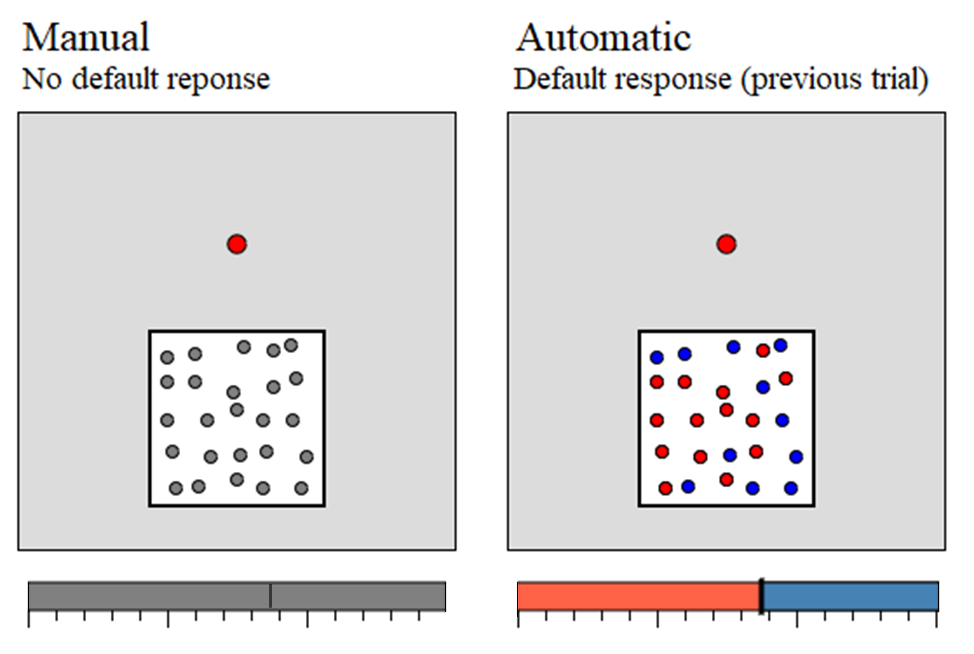
\includegraphics[width=0.50\textwidth]{trial-design}
    \caption{Experimental display}{Task display. Every trial, a red or blue dot floats out of an urn and participants adjust the slider to represent their estimate of the proportion of red to blue dots in the urn.}
    \label{fig:taskdisplay}
\end{figure}



Participants also completed 30 practice trials. Instead of estimating the actual Bernoulli parameter, participants aligned their estimates with a grey line generated randomly. This was to measure their tolerance for imprecision. Errors recorded on practice trials were taken as evidence that some participants did tolerate error from precise slider alignment (and so there may be noise in Manual participant responses).  Of these 89 participants, 61 tolerated some error on practice trials. Median number errors was 2, and mean error size was 1.5\%.







Participants were randomly assigned into two conditions (37 Manual, 52 Automatic). The Automatic condition was designed to mimic previous research. Automatic condition participants were given their last response as their default response. In contrast, in the Manual condition, participants were given no default response. On each trial, the slider began grey and was without an initial position. The previous estimate was shown with a grey line (as in the practice trials). To maintain their response from the previous trial, participants needed to align a red/blue border they introduce with the prior response indicator. Participants could either click and drag the slider, or click anywhere on the slider and the response bar would snap to that position. If participants failed to adjust the slider before attempting to move to the next trial, red text would prompt them to do so. A quick manipulation check determined that Manual participant average reaction time (M = 2365.7, SD = 735.94) was longer than that of Automatic participants (M = 1432.96, SD = 888.27; \textit{t}(84.91) = 5.4, p \(<\) 0.001). 

The dependent variable of interest for these analyses was number of adjustments. An adjustment was any change in estimate of the Bernoulli parameter from one trial to the next. Adjustment size was measured in slider increments. Response maintenance was an adjustment of size zero, and was not considered an adjustment in the following analyses. Adjustments were also re-coded. For the following analyses, positive adjustments are "sample-consistent" and negative adjustments are "sample-inconsistent". For positive adjustments, new Bernoulli estimates have changed to increase the probability of the latest dot colour.

\section{Results}\label{sec-results}

Our results show that both conditions exhibited large heterogeneity in updating frequency. In the Manual condition, the removing of the default response disposed participants to update more frequently, but also introduced noise. Importantly, in a subset of participants, this manipulation did not eliminate step-wise updating completely. Participants can exhibit step-wise response patterns even when they are forced to make a manual report on every trial. On the other hand, participants given a default response may exhibit near-constant updating. This demonstrates substantial individual differences in intentional updating frequency.








\subsection{Requiring trial by trial responses does lead to more frequent updating}

The Manual condition (M = 708.24, SD = 205.41) did update on more trials than the Automatic condition (M = 307.71, SD = 265.63; Figure \ref{fig:gross-diff}). An independent samples t-test confirmed a significant difference in the number of non-zero adjustments (\textit{t}(87) = 7.68, p \(<\) 0.001). However, rather than these extra adjustments necessarily reflecting true changes to their estimates of the Bernoulli parameter, they may simply reflect noise; participants may have been imprecise in where they placed their mouse click on the previous-response line when they intended to maintain a response.

\begin{figure}[htp]
\centering
\begin{knitrout}
\definecolor{shadecolor}{rgb}{0.969, 0.969, 0.969}\color{fgcolor}
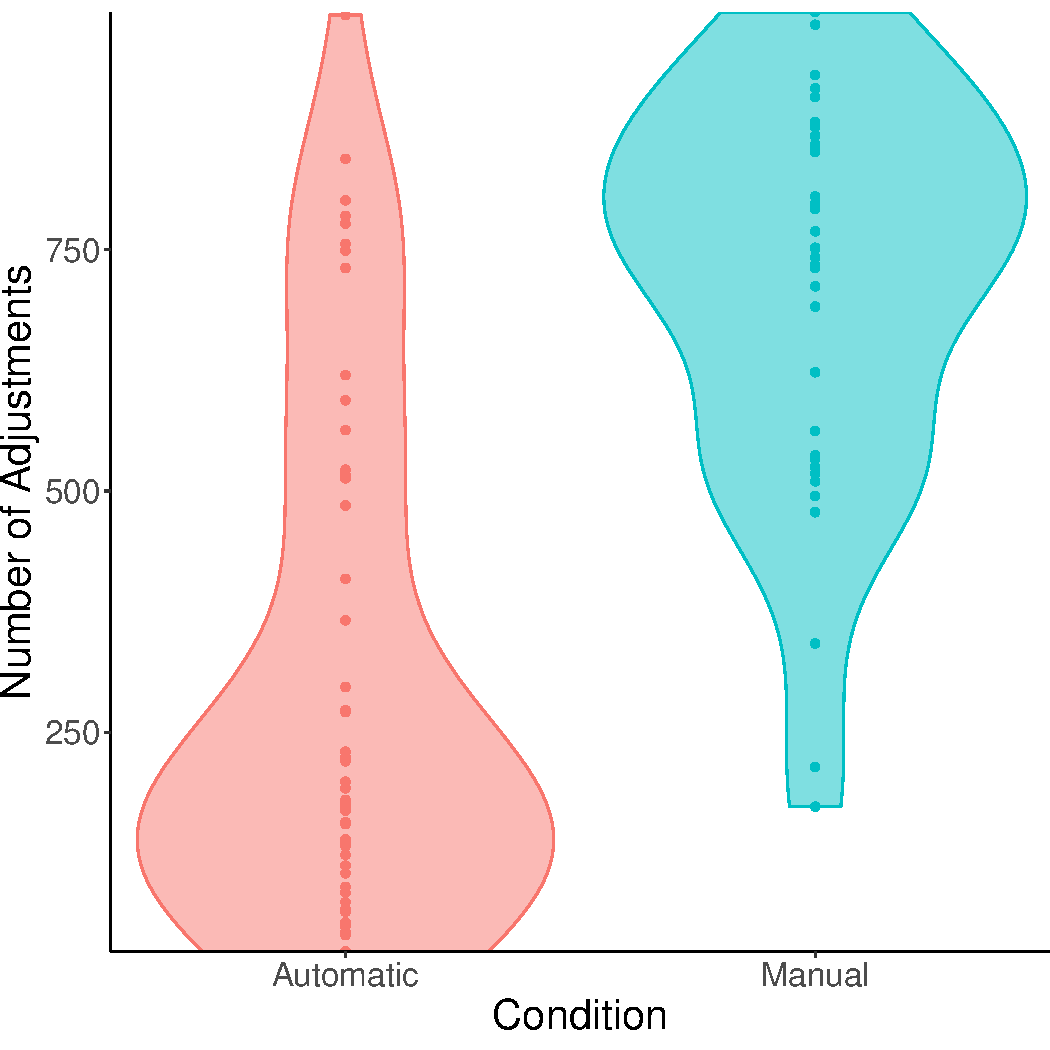
\includegraphics[width=0.5\textwidth]{figure/unnamed-chunk-9-1} 
\end{knitrout}
\caption{Boxplot showing group differences in total number of adjustments. Manual condition participants did make more adjustments, but these were disproportionately evidence consistent suggesting they were not simply due to noise and imprecise estimates.}
\label{fig:gross-diff}
\end{figure}






To determine whether additional adjustments made by the Manual condition were noise or true new updating events, we started with a set of simple t-tests. Consistent with there being added noise, participants in the Manual condition made a higher proportion of sample-inconsistent adjustments (M = 0.37, SD = 0.25) (relative to sample-consistent adjustments) compared to the Automatic condition (M = 0.23, SD = 0.37), \textit{t}(86.89) = 2.08, p = 0.041. However, these additional adjustments could not have been solely a reflection of added noise. The adjustments Manual participants made (after subtracting out average number automatic adjustments) were more often sample-consistent (M = 260.98, SD = 198.72) than sample-inconsistent(M = 139.56, SD = 101.95), \textit{t}(53.72) = -3.31, p = 0.002.

The differences detected above establish that the Manual condition distributed their responses more about zero (made noisier estimates) but also made more small adjustments consistent with the evidence (added updating events). This change in updating behavior is explored below by comparing the fit of different mixture models (Figure \ref{fig:numadj}). Automatic participant adjustment distributions were modeled first and then these models were compared to those of the Manual condition. 

Automatic participants were modeled using the equation below. P(x) is the probability of an adjustment of size x. For Automatic participants, this probability was hypothesized to be made up of the sum of two different Gaussian distributions. According to the step-wise pattern identified in previous research, the large majority of responses should be response-maintenance (designated by subscript \emph{m}) and other responses should be above-threshold updating events (subscript \emph{a}). 

\begin{equation}
  P(x) = P_m \cdot \mathcal{N}(0,\,\sigma_{m}^{2}) + P_a \cdot \mathcal{N}(\mu_{a},\,\sigma_{a}^{2})\,
\end{equation}

Model fitting was done using the nls function from the base R stats package, using the "port" algorithm. The 998 adjustments per each trial were converted to histograms for the model fitting. Each data point was the number of adjustments made per adjustment size.

Model comparison began with a simple check. Every Automatic participant was first fit to a single Gaussian distribution (two free parameters) and this fit was compared to that of the two Gaussian mixture model discussed above (five free parameters). For this second two-Gaussian model, the mean of one Gaussian was fixed at zero to represent response maintenance, and the mean of the other Gaussian was free to vary. For both Gaussians, the standard deviation and mixture coefficients were fit as free parameters. Model fit robustly improved. Out of the 52 participants, 52 showed AIC decreases (M = 441.61, SD = 389.89).

As discussed above, Manual participants decreased response maintenance and increased adjustments compared to Automatic participants. We assumed that noisy responses would redistribute response-maintenance symmetrically around zero, resulting in a wider Gaussian with a larger standard deviation. In contrast, new updating events would be more likely to be in line with recent evidence and therefore should be positively biased. New updating events were thus represented by adding a third Gaussian to the two-Gaussian mixture model presented above. In the equation below, the subscript \emph{b} refers to these updates having otherwise been \emph{below} the motor-response threshold for Automatic participants.

\begin{equation}
  P(x) = P_m \cdot \mathcal{N}(0,\,\sigma_{m}^{2}) + P_a \cdot \mathcal{N}(\mu_{a},\,\sigma_{a}^{2}) + P_b \cdot \mathcal{N}(\mu_{b},\,\sigma_{b}^{2})\,
\end{equation}

The two-Gaussian mixture model used to model Automatic participants was refit to Manual participants but with two instead of five free parameters. This is because the second Gaussian (representing above motor-threshold updating events) was estimated from Automatic participant data and was then fixed for every Manual participant. The fixed second Gaussian was estimated by fitting the two-Gaussian model to the entire Automatic condition, collapsing across all participants. For Manual participants, this left only the standard deviation and mixing coefficient of the first Gaussian (representing response maintenance) free to vary.  Consistent with the noise prediction, the standard deviation of the Gaussian model increased (from an average of 0.43 to 2.47, \textit{t}(49.78) = -2.86, p = 0.006).

In contrast to added noise, true updating events should be in line with recent evidence. A third Gaussian was added to model Manual participant adjustments, with three new parameters to fit: a new variable mean, standard deviation, and mixture coefficient. The standard deviation and mixture coefficient of the first Gaussian were allowed to vary again, resulting in a five-parameter model. On aggregate, collapsing across the entire Manual condition to fit the mixture models, model fit improved and resulted in a AIC decrease of 782.27. Individual participants were also fit to this model. Adding this third Gaussian to the mixture model for Manual participants decreased AIC values for 33 of the 35 Manual participants (M = 291.83, SD = 241.58). 

To determine how specific the improved model fitting was to Manual participants, the same two and three-Gaussian models were also fit to Automatic participants. AIC decreased by 3.22 for the aggregate models. Per individual cases, out of 48 Automatic participants, 16 decreased AIC (M = 107.79, SD = 204.89).





This sequential model fitting procedure should be understood as approximately representing the two substantial ways in which Manual participants made more adjustments; their estimates were noisier and they made more frequent minor adjustments. This should not be mistaken for evidence that Manual participant responses were truly trimodal, nor strategy uniform. Nonetheless, adopting the appropriate skepticism with these imprecise models, they can be used to estimate the proportion of responses attributable to each of three hypothesized sources. On average, Manual participant responses were made up of 34.49 \% (283.89) response maintenance, 30.74 \% (286.24) new below-motor threshold updating events (average size 1.1\%), and 34.77 \% (253) updating events already accounted for by Automatic participant adjustments (average size 3.94\%). 

While our three-Gaussian modelling procedure accounts for group-level variance, individual participants vary. The median estimated mean adjustment size (0.79) was within the expected range to represent new below-threshold small updating events. However values spanned from -3.9 to 9.46 (IQR = 2.41). We take negative means to indicate that the model underestimated sample-inconsistent values more than it underestimated sample-consistent adjustments (as would be the case with added noise coupled with infrequent updating). Large positive values indicate participants who made more large sample consistent adjustments than the model predicted. Thus, while the group-level model captures well the general differences between the groups, there remained substantial individual differences.


\begin{figure}[htp]
\centering
\begin{knitrout}
\definecolor{shadecolor}{rgb}{0.969, 0.969, 0.969}\color{fgcolor}
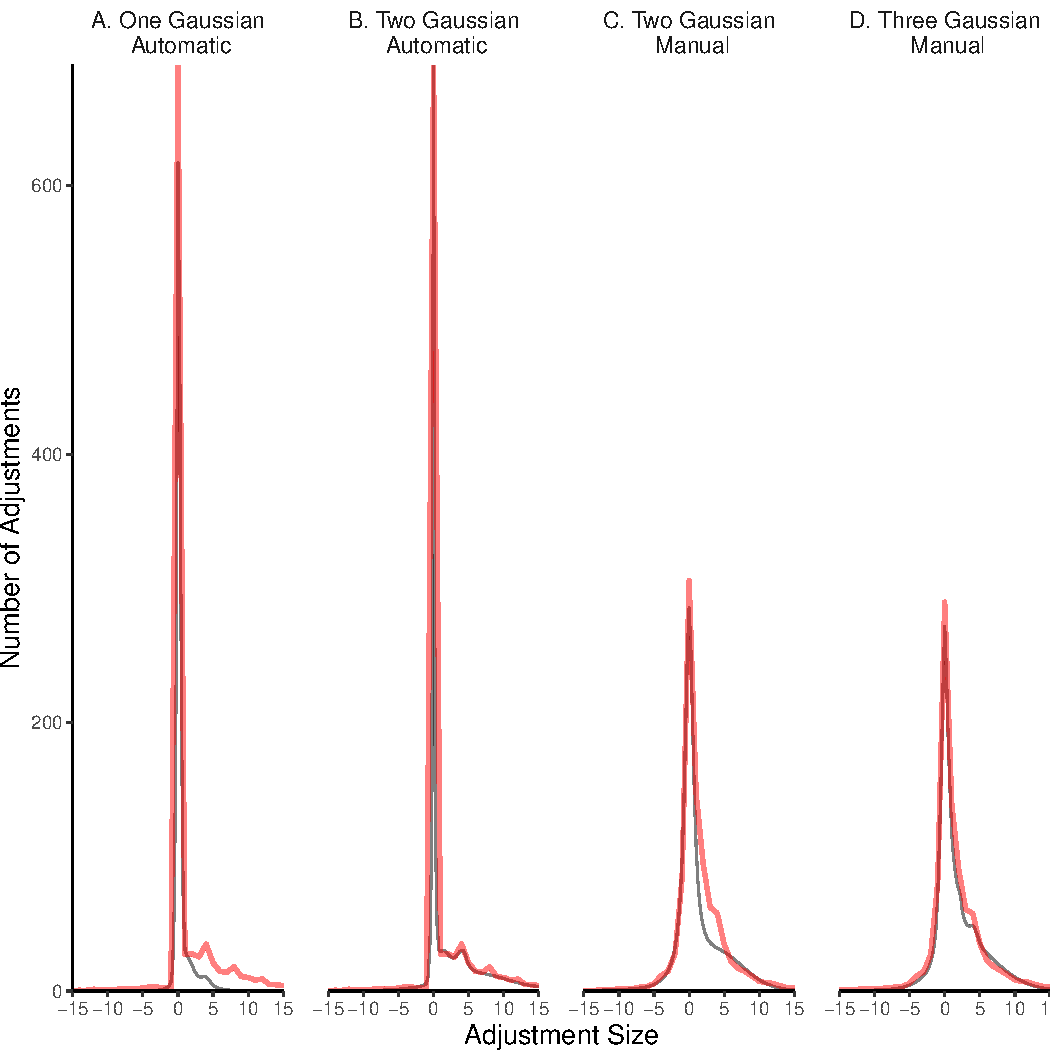
\includegraphics[width=0.8\textwidth]{figure/unnamed-chunk-12-1} 
\end{knitrout}

\caption{Model fits for number of adjustments over adjustment size. Negative-sign adjustments are sample-inconsistent. Positive-sign adjustments are sample-consistent. Window is restricted to adjustments under 15 percentage points. The red line represents the actual mean number of adjustments made by either condition.  The black line represents the estimated mean number of adjustments generated from averaging over individual model fits. (A.) Automatic participant data modeled using only a single Gaussian. (B.) Automatic participant data modeled using two Gaussians where one had a mean fixed at zero and the other was allowed to vary. These two distributions respectively represent two different types of responses: maintenance and updating events. (C.) Manual participant data modeled by refitting  parameters from model B. This represents how redistribution of responses would occur under the noise hypothesis. Only the standard deviation and scale of the one Gaussian with the mean fixed at zero were allowed to vary. (D.) Manual participant data modeled again by refitting the parameters of model B and adding a third new Gaussian distribution to represent added true new updating events.}

\label{fig:numadj}
\end{figure}


\subsection{Updating is individually heterogeneous}

A presumption of many models concerning decision making contain an implicit assumption of group homogeneity. However, previous research has shown that there are great individual differences in the generation of probability estimates \cite{khaw2021}. Consistent with this research, we found wide variation in individual response patterns that are not well explained by group trends.





As discussed above, the Manual and Automatic conditions performed distinctively. Manual participants updated more often and were noisier than Automatic participants. 

\begin{figure}[htp]
\centering




\begin{knitrout}
\definecolor{shadecolor}{rgb}{0.969, 0.969, 0.969}\color{fgcolor}
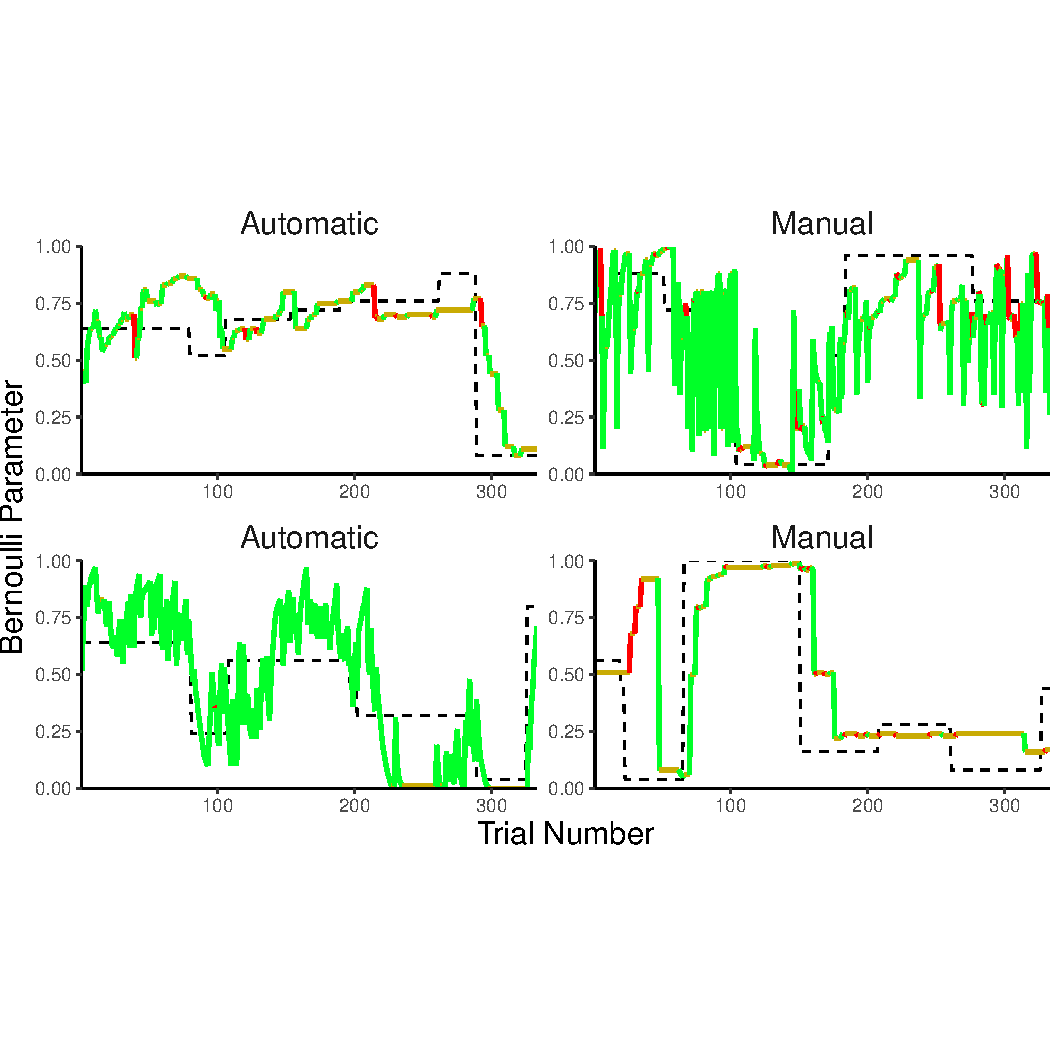
\includegraphics[width=0.9\textwidth]{figure/unnamed-chunk-16-1} 
\end{knitrout}
\caption{Representative cases (first row) and extreme cases (second row) of response patterns in Block 1 for Automatic and Manual participants. Participants in the first row represent typical cases; they each made the median number of adjustments per their group. Participants in the second row represent atypical and extreme cases of meticulous updating. The dotted line represents the true Bernoulli parameter. The coloured line represents the participant estimate. Where the line is green, the adjustment was sample-consistent; where the line is red it was inconsistent. Where the line is yellow, there was no change from one trial to the next (i.e. response maintenance).}
\label{fig:representative_ppts}
\end{figure}


However, some Manual condition participants (those required to make a mouse based report on every trial) made \emph{fewer} adjustments than the average Automatic condition participant demonstrating clear cases of spontaneous meticulous stepwise patterning. The rarity of these extreme cases is visible in Figure \ref{fig:gross-diff}, and illustrated by the fact that, of 84 Manual participants in our original sample, 6 participants made fewer adjustments than the average Automatic participant. These cases of the rarest updating in the Manual group (1/5 trials) also reflects substantially higher updating rates than those observed in previous research \cite{gallistel2014, ricci2017,khaw2017}. Complementarily, there were Automatic condition participants with meticulous frequent updating that exceeded the average Manual condition participant (Figure \ref{fig:representative_ppts}). The number adjustments for Automatic participants ranged from  23 to 993, and for Manual participants ranged from 173 to 996 \footnote{Plots per every individual participant, as in Figure \ref{fig:representative_ppts},  are provided in supplementary material (https://github.com/jschirme/Bernoulli-Estimation/tree/main/Supplementary)}.



\section{Discussion}\label{sec-disc}

There is debate over how people integrate new samples to update estimates of probabilities. In trial-by-trial models, flexibility is achieved by having samples pull probabilities towards them, weighting samples by recency \citep{forsgren2023further,nassar2010,nassar2012,brown2009,krugel2009,steyvers2005}. In change-point detection models, flexibility is achieved by detecting distinct change-points \citep{gallistel2014}.

Major support for change-point detection models comes from step-wise response patterns \citep{gallistel2014, ricci2017}. However, this evidence may be confounded. In this research, when participants are given their last response as a default response it is easier to make no response than a small adjustment. Our experiment was designed to remove this confound. The Manual condition had participants respond every trial with no default provided, thus removing any additional motor cost to updating.

Manual participants did make more adjustments. This appeared to be both due to added noise and added new updating events. Regarding noise, the best-fit response-maintenance Gaussian for Manual participants had a wider standard deviation than did the Gaussian for Automatic participants. This wider variance suggests that attempts to maintain a response became scattered. While this has the unfortunate consequence of making updating intention more difficult to isolate, it is consistent with other research which suggests an element of arbitrary randomness in participant reports of their estimates of probabilities. Even when participants are exposed to the same deterministic sequence of samples, their estimates of the underlying probabilities vary \citep{prat2024}. 

On top of noise, it appears new minor updating events were also added to Manual condition adjustments. Adding a third Gaussian to the model, representing new updating events, substantially improved model fit. Thus, removing the motor cost did appear to increase updating.

However, stepwise behavior did not disappear in the Manual condition. A minority of meticulous Manual participants on the more extreme ends of updating infrequency, unprompted, elected to maintain their response the vast majority of trials. This \emph{more} effortful stepwise behavior must reflect intention and cannot fully be explained by motor cost. 

However meticulous stepwise updating was rare in the Manual group and even in the Automatic group it was not universal. In the Automatic condition, some participants showed striking sawtooth pattern behavior, updating their responses in line with recent events on near every trial. This is also clearly effortful and intentional behavior opposite to intermittent updating. It demonstrates a complementary capacity for trial by trial updating.

There may yet be space for both accounts. Great within-group variability highlights the potential for hybrid models that blend multiple mechanisms and express themselves in varying degrees in different individuals. The thrust of the current research is to demonstrate that stepwise behavior found in previous research is not universal but in some can be meticulous and intentional and therefore is not fully explained by a pervasive motor-cost confound. Future models directed at explaining probability estimation must account for substantial heterogeneity in updating frequency. 

The underlying mechanism by which probability estimates are generated is not investigated here. It is worth noting that both traditional trial-by-trial models and change-point detection models can grow to accommodate this wider range of response-frequences. A hybrid delta-updating model, for instance, was proposed by \cite{forsgren2023further}. In this model, probability estimates are generated using the delta-updating model, but a threshold-procedure prevents continuous updating. Likewise, the change-point detection model proposed by \cite{gallistel2014} (If It Ain't Broke) can include frequent incremental updating between detected change-points as each small adjustment improves the precision of the running estimate.

In our work, remarkable intentional behavior seems to support both extreme forms of trial-by-trial and change-point detection updating. Intermittent updating cannot be fully be explained by motor-cost to updating, but not all updating is intermittent. People can spontaneously generate the intentional choice to update frequently in small amounts or infrequently in larger steps.


\section{Declarations}

\begin{itemize}
\item Funding:
This work was supported by NSERC.
\item Conflict of interest:
The authors have no competing interests to declare that are relevant to the content of this article.
\item Ethics approval:
The procedures and methodology for this study was cleared by the Office of Research Ethics  of the University of Waterloo  (ORE 42844).
\item Consent to participate:
All participants in this research gave informed consent before starting the experiment.
\item Consent for publication:
Not applicable
\item Availability of data and materials:
The datasets generated during and/or analysed during the current study will be made available in the OSF repository. 
\item Code availability:
The code used to analyze the data will be made available in the OSF repository. 
\end{itemize}

\subsection{Open Practices Statement}

A public repository for data,, analyses and supplementary materials is at the link: https://osf.io/8nc5d/. This experiment was not preregistered.

\bibliography{sn-bibliography}% common bib file

\end{document}

%%% Local Variables:
%%% mode: LaTeX
%%% TeX-master: t
%%% End:
